\documentclass[12pt]{article}

\usepackage[letterpaper,margin=1in]{geometry}

\setlength{\parindent}{0pt}

\usepackage{amssymb}
\usepackage{amsmath}

\usepackage{multicol}

\usepackage{tikz}

\newcommand{\headerText}{
  MA 237 | Spring 2018 | Dr. Clontz
}

\usepackage{fancyhdr}
\pagestyle{fancy}
\renewcommand{\headrulewidth}{0pt}% Default \headrulewidth is 0.4pt
\renewcommand{\footrulewidth}{0pt}% Default \footrulewidth is 0pt
\chead{\footnotesize\bf\headerText}
\cfoot{}

\newcommand{\csch}{\operatorname{csch}}
\newcommand{\sech}{\operatorname{sech}}

\newcommand{\issuesMark}{{\fontencoding{U}\fontfamily{futs}\selectfont\char 66\relax}}





\begin{document}


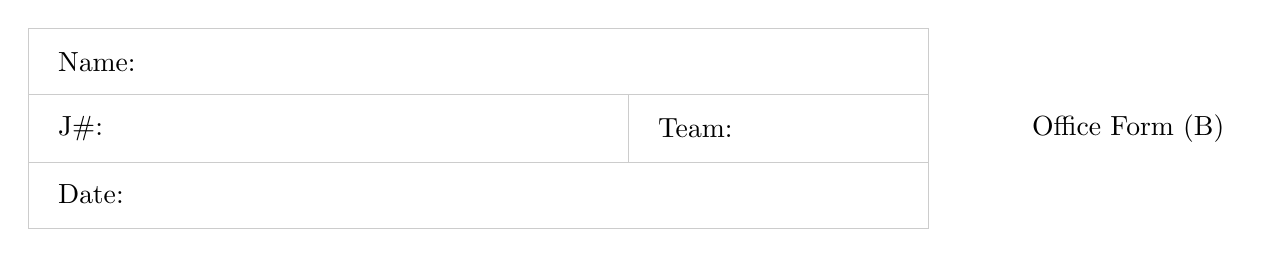
\begin{tikzpicture}[x=1in,y=1in]
  \draw[color=black!20] (0,0) rectangle (4.5,1);
  \draw[color=black!20] (0,0.67) -- (4.5,0.67);
  \draw[color=black!20] (3,0.33) -- (3,0.67);
  \draw[color=black!20] (0,0.33) -- (4.5,0.33);

  \node[anchor=west] at (0.1,0.83) {Name:};
  \node[anchor=west] at (0.1,0.5) {J\#:};
  \node[anchor=west] at (3.1,0.5) {Team:};
  \node[anchor=west] at (0.1,0.17) {Date:};

  \node at (5.5,0.5) {Office Form (\issuesMark{})};
\end{tikzpicture}

\vspace{1em}

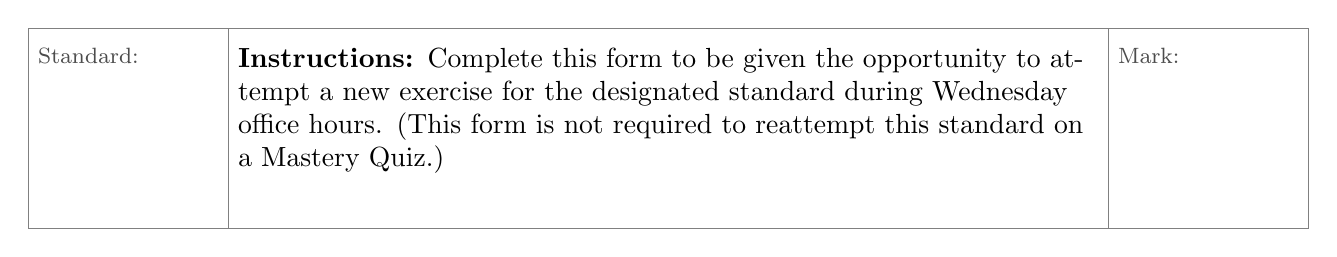
\begin{tikzpicture}[x=1in,y=1in]
  \draw[color=black!50] (0,0) rectangle (6.4,1);
  \draw[color=black!50] (1,0) -- (1,1);
  \draw[color=black!50] (5.4,0) -- (5.4,1);

  \node[anchor=north west,color=black!70] at (0,0.95) {\footnotesize Standard:};
  \node[anchor=north west,text width=4.3in] at (1,0.95) {\textbf{Instructions:} Complete this form to be given the opportunity to
  attempt a new exercise for the designated standard during Wednesday
  office hours. (This form is not required to reattempt this
  standard on a Mastery Quiz.)};
  \node[anchor=north west,color=black!70] at (5.4,0.95) {\footnotesize Mark:};
\end{tikzpicture}


\renewcommand\labelitemi{\(\square\)}
Mark all that apply.
\begin{itemize}
  \item I have previously attempted this standard on a Mastery Quiz
        and received a mark of \issuesMark{} or better (\(\ast\),\checkmark{}).
  \item I scored at least 70\% on the individual readiness assurance test (iRAT)
        for the most recent module, or I have reviewed all the
        readiness assurance resources for the module since the iRAT
        (and can answer relevant questions related to those materials).
  \item I have been present in class and on time for the last three class days,
        or my tardiness/absences have been for excusable reasons.
  \item My team has satisfactorily participated in all class assignments
        for the past three class days, such as:
    \begin{itemize}
      \item any team readiness assurance tests
      \item activities completed on the whiteboard (not individual notes)
            and uploaded to Google Drive
    \end{itemize}
  \item I have completed at least three homework exercises relevant to the
        standard designated above, written on or attached to this form.
        (These standards may be from any source, such as the textbook,
        internet, or old quizzes, as long as they match the designated
        standard.)
\end{itemize}

If you meet all these requirements,
bring this form to the instructor's Wednesday office hours. This counts
as one of your ten submissions for the next Mastery Quiz.

\vspace{1em}

If the attached exercises have been worked correctly, you will be given
a new exercise to complete, which will be marked immediately. If you
receive a \checkmark{}, you may not reattempt this standard on the next
Mastery Quiz (you must wait another week).

\vspace{1em}

If the attached exercises have not been worked correctly, or the
new exercise was not marked with a \checkmark{}, you may reattempt
this standard on the next Mastery Quiz.


\end{document}
